\subsection{Analisis Kebutuhan Sistem}

% bingung nulis apa lagi disini
Pada bagian \ref{subsec:analisis-alternatif-solusi}, telah disimpulkan pilihan alternatif yang akan digunakan dalam membangun sistem. Alternatif-alternatif solusi yang digunakan akan menjadi komponen yang saling berinteraksi dalam sistem Smart Contract Discovery untuk menyediakan fungsionalitas yang terpadu. Pada bagian ini akan diuraikan lebih lanjut mengenai sistem yang akan dibangun sehingga dapat memberikan panduan dalam fase pengembangan sistem. Penjelasan ini mencakup deskripsi sistem, karakteristik pengguna, kebutuhan fungsional dan non-fungsional, serta model use case yang akan digunakan dalam sistem.

\subsubsection{Deskripsi Sistem}
% penjelasan gambaran umum sistem, komponen utamanya apa aja
% buat diagram UML gambaran umum
% Jelaskan tujuan utama sistem (misalnya: "Membangun sistem pencarian smart contract berbasis semantik untuk meningkatkan efisiensi pengembangan dApps").

Solusi yang akan dikembangkan adalah sebuah sistem Smart Contract Discovery yang bertujuan untuk menyediakan \textit{platform} pencarian Smart Contract dalam Blockchain Ethereum berbasis semantik memanfaatkan LLM dan RAG. Sistem akan dibagi menjadi beberapa komponen utama yang saling berinteraksi untuk menyediakan fungsionalitas yang terpadu. Komponen utama sistem adalah sebagai berikut:

\begin{enumerate}
  \item Komponen Ekstraksi Data
  \item Komponen Penyimpanan Data
  \item Komponen \textit{Semantic Enrichment}
  \item Komponen Pencarian
  \item Komponen Antarmuka Pengguna
\end{enumerate}

\begin{figure}[ht]
	\centering
	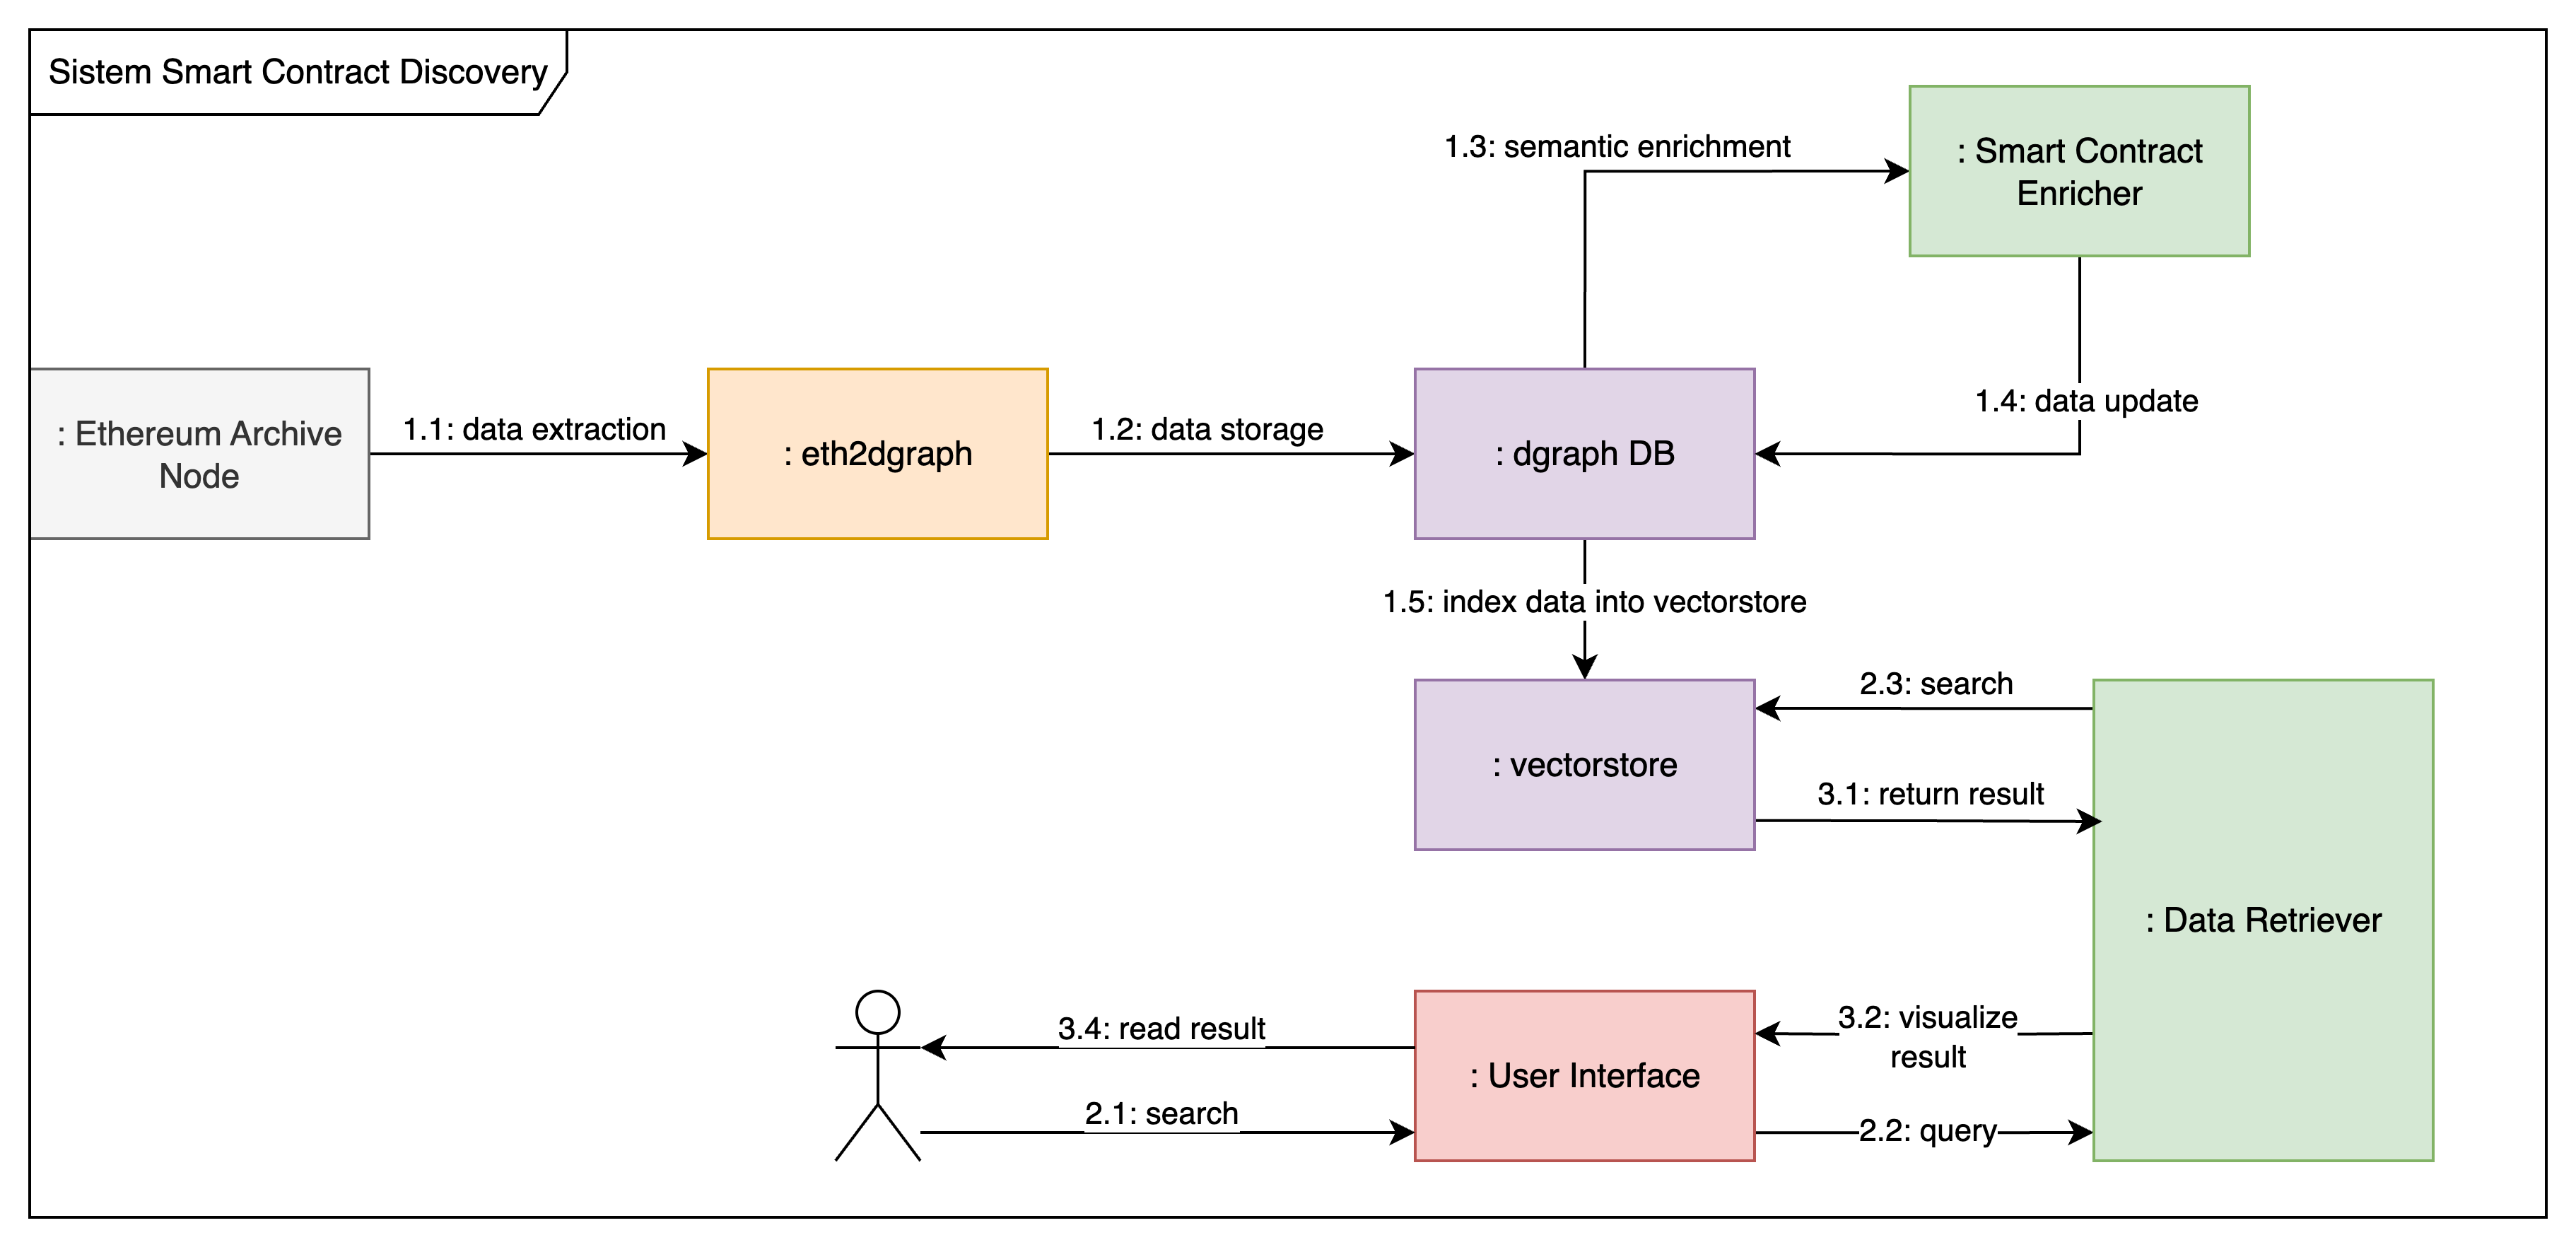
\includegraphics[width=1\textwidth]{resources/chapter-3/komponen-utama-new.png}
	\caption{Gambaran Umum Interaksi Komponen Utama Sistem}
	\label{image:komponen-sistem}
\end{figure}

\begin{figure}[ht]
	\centering
	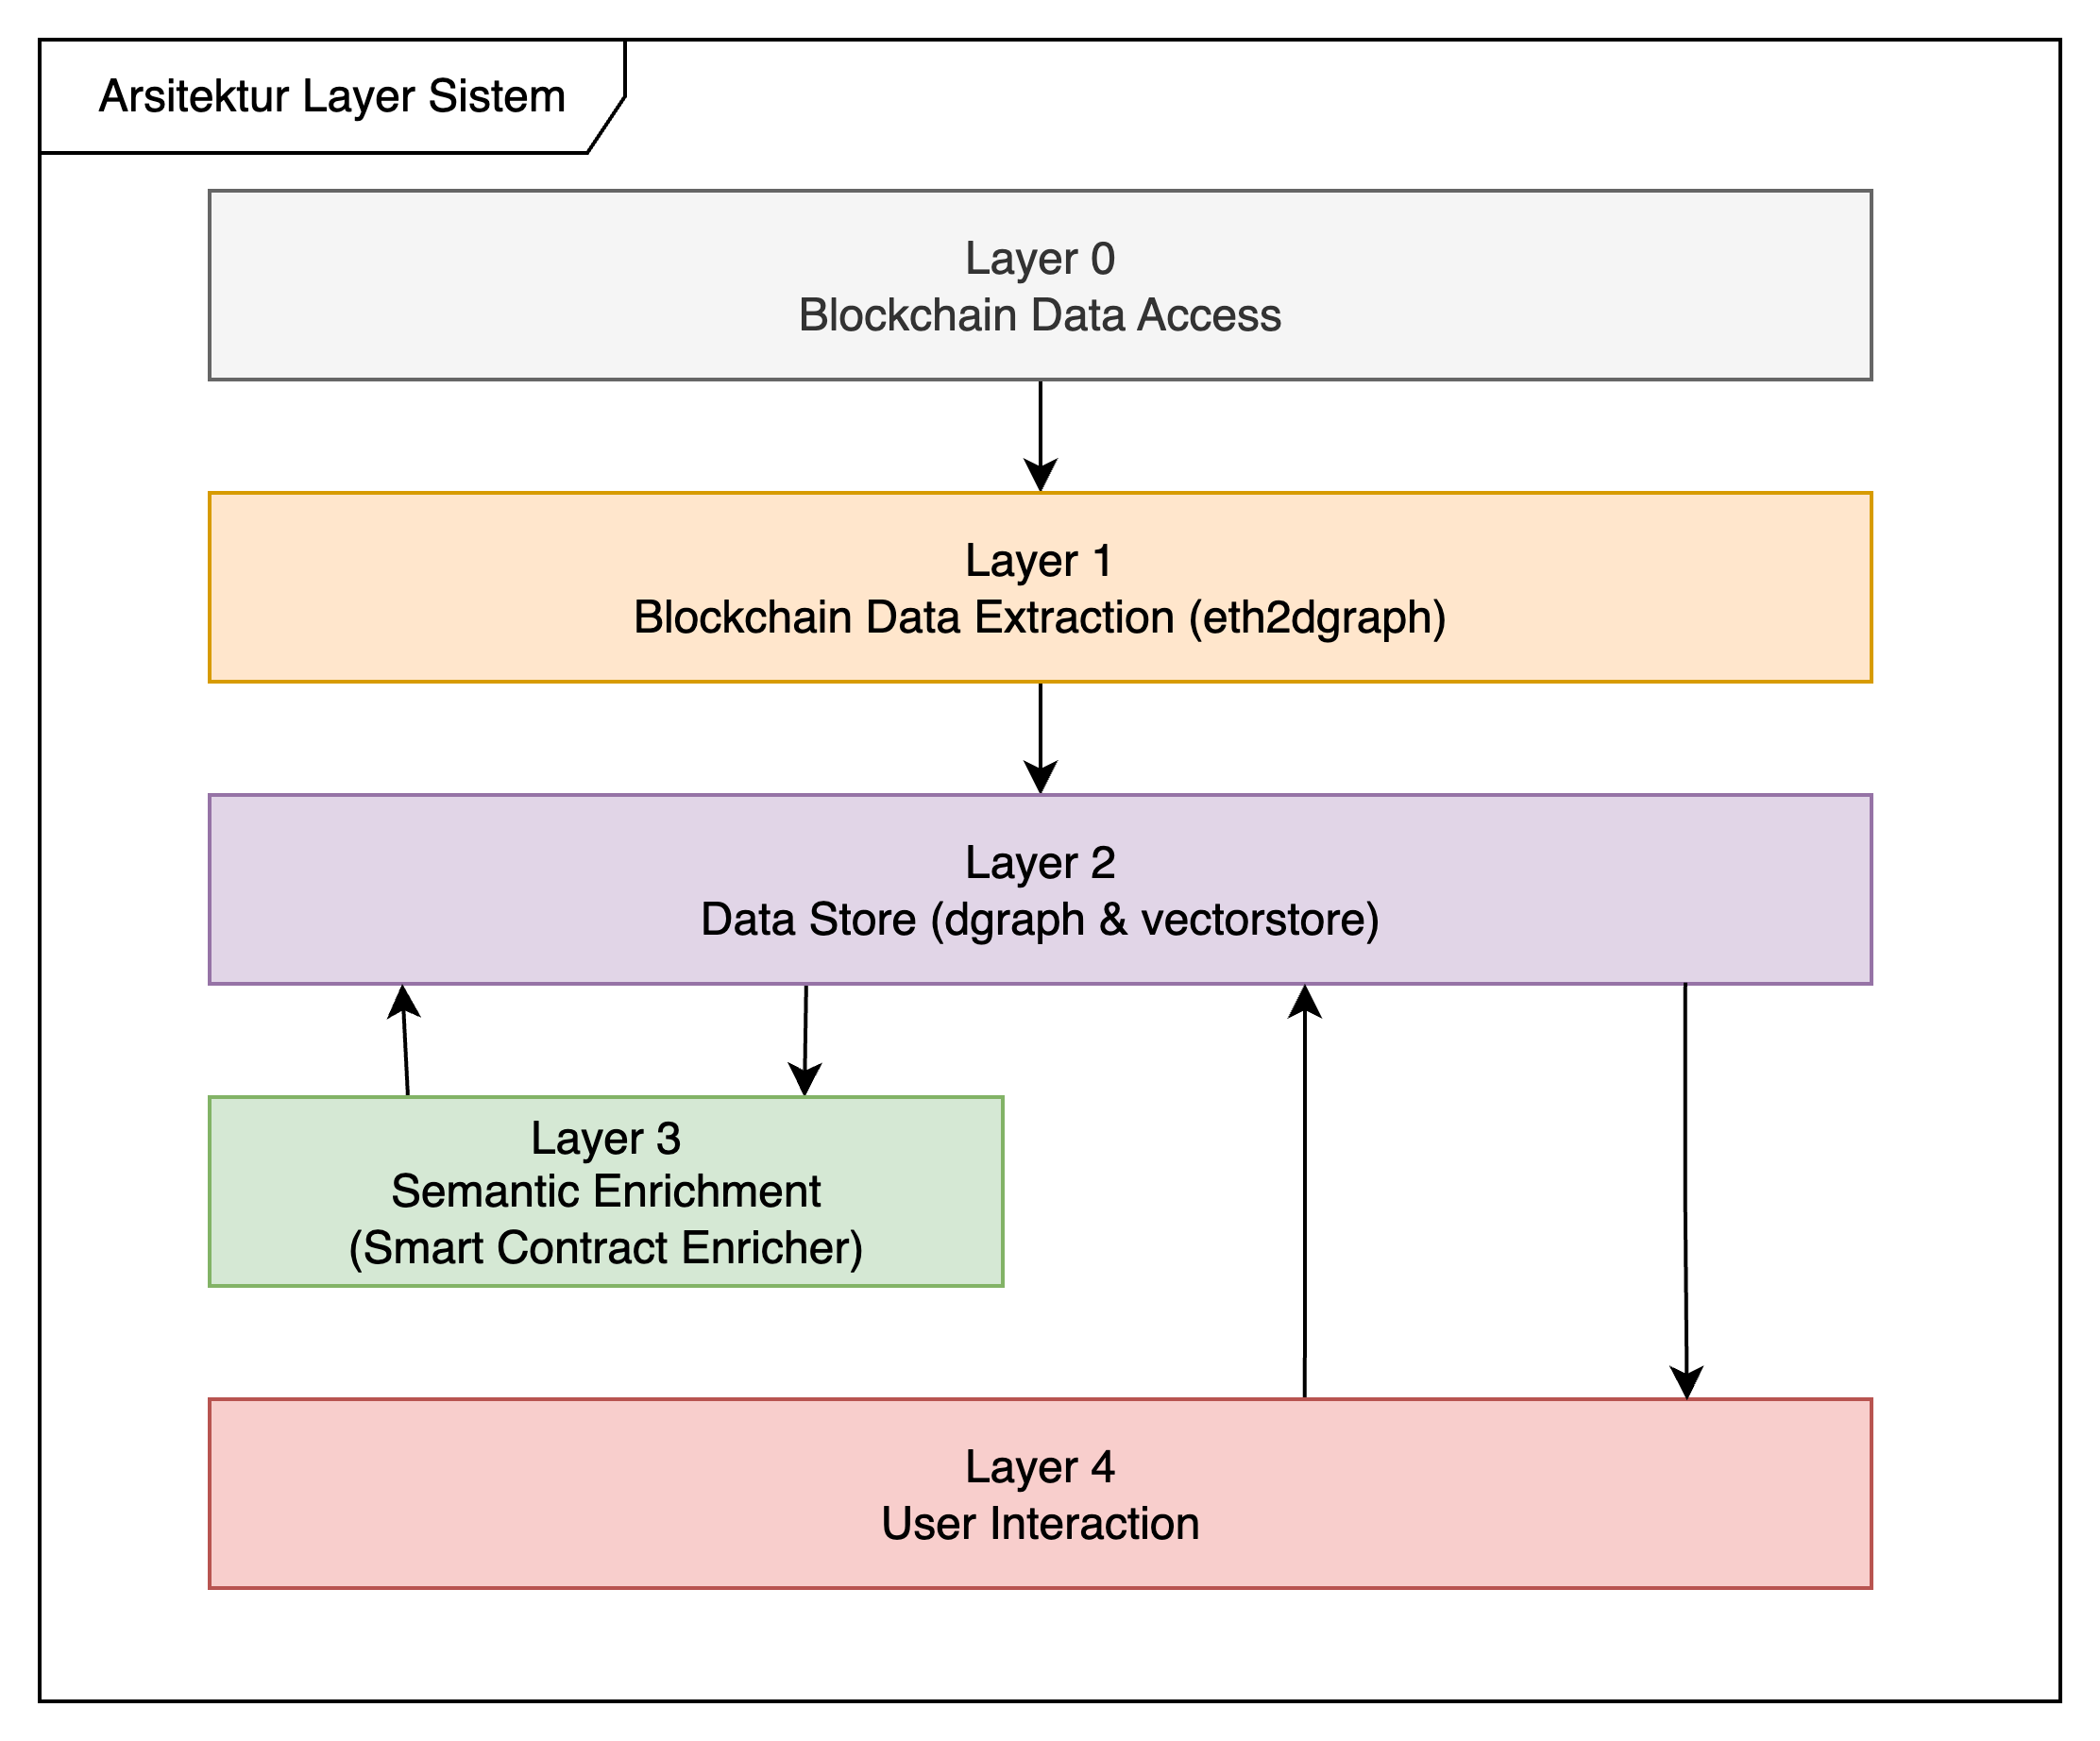
\includegraphics[width=0.7\textwidth]{resources/chapter-3/layer-arsitektur-new.png}
	\caption{Gambaran Arsitektur Layer Sistem}
	\label{image:layer-arsitektur}
\end{figure}

% Ethereum Archive Node → eth2dgraph (ekstraksi) → Dgraph (penyimpanan) → LLM (semantic enrichment) → Dgraph (update) → RAG (query).  

Gambar \ref{image:komponen-sistem} dan gambar \ref{image:layer-arsitektur} menunjukkan gambaran umum alur kerja sistem. Sistem ini akan melakukan ekstraksi data dari Ethereum Archive Node menggunakan \textit{eth2dgraph} dan menyimpannya dalam Dgraph. Setelah itu, sistem akan melakukan \textit{semantic enrichment} menggunakan LLM untuk memperkaya deskripsi dan metadata Smart Contract, lalu memperbarui data di Dgraph. Sebelum data dapat dilakukan query menggunakan RAG, akan dilakukan indexing data menjadi bentuk vectorstore. Terakhir, sistem akan menggunakan RAG untuk melakukan pencarian berdasarkan kebutuhan pengguna. 



\subsubsection{Karakteristik Pengguna}

Sistem ini hanya akan digunakan oleh satu jenis pengguna, yaitu User yang ingin mencari Smart Contract. Belum ada mekanisme yang membutuhkan campur tangan pengguna lain, seperti pengembang atau administrator. Pengguna dapat melakukan pencarian Smart Contract berdasarkan kebutuhan fungsionalitas yang diinginkan. Pengguna tidak perlu memiliki pengetahuan teknis yang mendalam tentang Smart Contract atau Blockchain untuk menggunakan sistem ini. Antarmuka pengguna dirancang agar mudah digunakan dan intuitif, sehingga pengguna dapat dengan mudah menemukan Smart Contract yang sesuai dengan kebutuhan mereka, dan menggunakannya, baik digunakan secara langsung, atau menjadi komponen di dalam aplikasi yang lebih besar.

\subsubsection{Kebutuhan Fungsional}

Sistem ini memiliki beberapa kebutuhan fungsional yang harus dipenuhi agar dapat berfungsi dengan baik. Kebutuhan fungsional ini mencakup semua fitur dan fungsi yang harus ada dalam sistem untuk memenuhi tujuan utama sistem. Berikut adalah daftar kebutuhan fungsional yang diidentifikasi:

% tabel
% \begin{table}[h]
% 	\caption{Kebutuhan Fungsional Sistem}
% 	\vspace{0.25cm}
% 	\begin{center}
% 		\begin{tabular}{|c|l|}
% 			\hline
% 			\textbf{ID} & \textbf{Penjelasan} \\ \hline
% 			F01 & User dapat melakukan input kebutuhan dalam bentuk \textit{Natural Language} \\ \hline
% 			F02 & User dapat mencari Smart Contract  \\ \hline
% 			F03 & Pengembangan Prototipe \\ \hline
% 			F04 & Pengujian Prototipe \\ \hline
% 			F05 & Evaluasi dan Perbaikan \\ \hline
% 		\end{tabular}
% 	\end{center}
% \end{table}

\subsubsection{Kebutuhan Non-Fungsional}

\subsubsection{Model Use Case}

Kebutuhan fungsional dan karakteristik pengguna yang dirumuskan dapat dimodelkan menjadi use case. Seperti pada gambar \ref{image:usecase}, Use case kemudian dapat dipetakan menjadi sebuah Use Case Diagram yang menghubungkan relasi antara aktor dengan use case yang berkolerasi. Diagram ini menggambarkan interaksi antara pengguna dan sistem, serta fungsi-fungsi yang tersedia dalam sistem. Diagram use case ini akan membantu dalam memahami bagaimana pengguna akan berinteraksi dengan sistem dan fitur-fitur apa saja yang harus ada dalam sistem. Use case dapat dilihat secara detail pada lampiran XX.

\begin{figure}[ht]
	\centering
	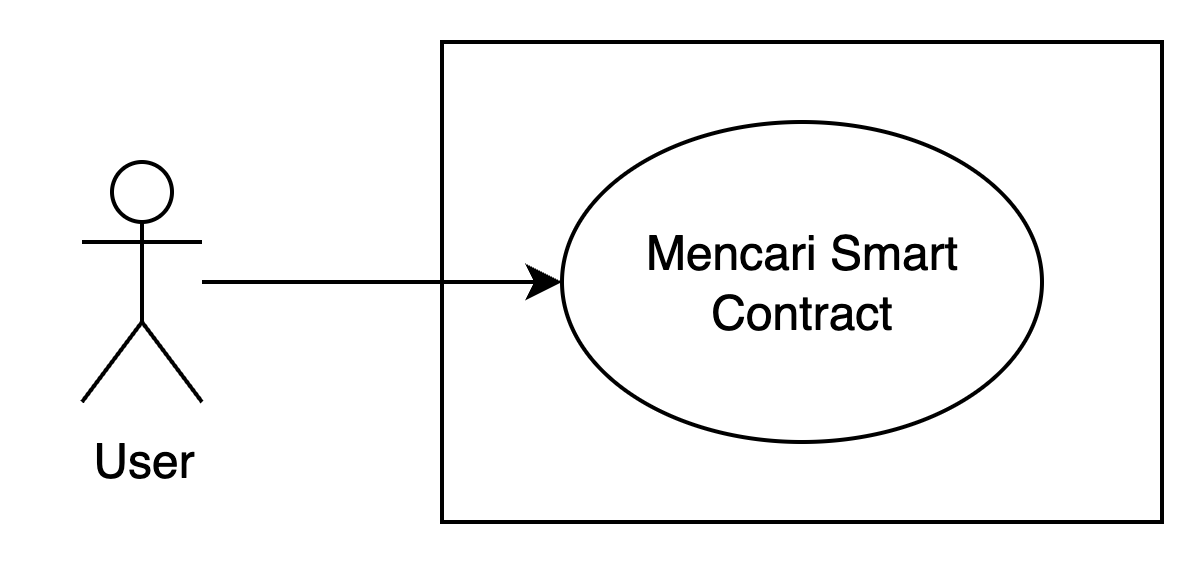
\includegraphics[width=0.7\textwidth]{resources/chapter-3/use-case.png}
	\caption{Use Case Diagram}
	\label{image:usecase}
\end{figure}

\subsubsection{Risiko dan Mitigasi}
